\RequirePackage{fix-cm}
\documentclass[10pt]{beamer}
\usepackage{adjustbox}

\usetheme{Madrid}
\usecolortheme{default}
\definecolor{moderncvgreen}{rgb}{0.35,0.70,0.30}
\colorlet{beamer@blendedblue}{moderncvgreen}
% \setbeamercovered{transparent}

\newcommand\topics[1][]{\textbf{topics}}
\newcommand\processes[1][]{\textbf{processes}}
\newcommand\institutions[1][]{\textbf{institutions}}

\newcommand\drift[1][]{\textbf{drift}}
\newcommand\layering[1][]{\textbf{layering}}
\newcommand\displacement[1][]{\textbf{displacement}}

\makeatletter
\newcommand\HUGE{\@setfontsize\Huge{50}{60}}
\makeatother

\usepackage{tikz}
\usepackage{tikzscale}
\usepackage{pgfplots}
\usetikzlibrary{shapes,positioning,calc,arrows.meta,decorations.pathmorphing,patterns,decorations, decorations.markings,arrows, shapes.geometric,fit,patterns.meta}
\usetikzlibrary{overlay-beamer-styles}
\usepackage{pgfplots}
\pgfplotsset{width=7cm,compat=1.16}
\usepgfplotslibrary{ternary}
\makeatletter
\pgfdeclaredecoration{penciline}{initial}{
    \state{initial}[width=+\pgfdecoratedinputsegmentremainingdistance,auto corner on length=1mm,]{
        \pgfpathcurveto%
        {% From
            \pgfqpoint{\pgfdecoratedinputsegmentremainingdistance}
                            {\pgfdecorationsegmentamplitude}
        }
        {%  Control 1
        \pgfmathrand
        \pgfpointadd{\pgfqpoint{\pgfdecoratedinputsegmentremainingdistance}{0pt}}
                        {\pgfqpoint{-\pgfdecorationsegmentaspect\pgfdecoratedinputsegmentremainingdistance}%
                                        {\pgfmathresult\pgfdecorationsegmentamplitude}
                        }
        }
        {%TO 
        \pgfpointadd{\pgfpointdecoratedinputsegmentlast}{\pgfpoint{1pt}{1pt}}
        }
    }
    \state{final}{}
}
\makeatother
\newcommand*{\coloremph}[2]{%
  \tikz[baseline=(X.base)] \node[rectangle, fill=#2, rounded corners, inner sep=0.3mm] (X) {#1};%
}
\usetikzlibrary{arrows}
\RequirePackage{fix-cm}
\usepackage{tikz-cd}
\usepackage{tikzpeople}
\usepackage{fontawesome5}

\usepackage{animate}

\usepackage{tabularx}
\usepackage{multirow}
\usepackage{multicol}
\usepackage{booktabs}

% \tikzset{
%   font={\fontsize{7pt}{9}\selectfont}}

 \usepackage{subcaption}
 \usepackage{amsmath,bm,amssymb}
 \usepackage{bbm}
 \DeclareMathOperator*{\argmax}{arg\,max}
 \DeclareMathOperator*{\argmin}{arg\,min}

\usepackage{hyperref}

\usepackage[backend=biber, style=authoryear, sortcites=false, uniquelist=false,natbib=true,doi=false,isbn=false,url=false,eprint=false,pagetracker, ibidtracker=constrict]{biblatex}
\DefineBibliographyExtras{french}{\restorecommand\mkbibnamefamily}
\AtEveryBibitem{\clearfield{entrysubtype}}
\AtEveryBibitem{\clearfield{pages}}
\renewcommand*{\nameyeardelim}{\addcomma\addspace}
\addbibresource{references.bib}
\renewcommand*{\bibfont}{\normalfont\fontsize{8}{10}\selectfont}

% \newcommand\Wider[2][3em]{%
% \makebox[\linewidth][c]{%
%   \begin{minipage}{\dimexpr\textwidth+#1\relax}
%   \raggedright#2
%   \end{minipage}%
%   }%
% }


%------------------------------------------------------------
%This block of code defines the information to appear in the
%Title page
\title[Inverse Problems for Philosophers] %optional
{
Inverse Problems for Philosophers
}
\subtitle{Bridging the gap between agent-based models and behavioral data}

\author[L.~Gautheron]
{Lucas~Gautheron\textsuperscript{1,2} (Ph.D. candidate)
}

\institute[IZWT, ENS] % (optional)
{
  %
  \inst{1}
  Interdisciplinary Center for Science and Technology Studies, Wuppertal, Germany\\
  \inst{2} Département d'Études Cognitives, École Normale Supérieure, Paris, France
}

\date[13/12/2024] % (optional)
{University of Bochum, December 2024}

%\logo{\includegraphics[height=1cm]{overleaf-logo}}

%End of title page configuration block
%------------------------------------------------------------



%------------------------------------------------------------
%The next block of commands puts the table of contents at the 
%beginning of each section and highlights the current section:

\AtBeginSection[]
{
  \begin{frame}
    \frametitle{Summary}

    % \textbf{Goal: understanding how the field of High-Energy physics adapts as a major research program loses its empirical support and content}
    \tableofcontents[currentsection]
  \end{frame}
}

% \AtBeginSubsection[]
% {
%   \begin{frame}
%     \frametitle{Summary}

%     % \textbf{Goal: understanding how the field of High-Energy physics adapts as a major research program loses its empirical support and content}
%     \tableofcontents[currentsection,currentsubsection]
%   \end{frame}
% }


\AtBeginSubsection[]
{
  \begin{frame}
    \tableofcontents[currentsubsection]
  \end{frame}
}


\begin{document}


%The next statement creates the title page.
\frame{
\titlepage
}

\begin{frame}{Summary}
    \tableofcontents
\end{frame}

\begin{frame}{Why should philosophers care about data?}
    \begin{itemize}
        \item<1-> Verify that models capture what is actually going on in the situations we are interested in.
        \item<2-> Robustness (insensitivity to model assumptions/parameters) is a fallible validation procedure: what if the outcome really is contingent on certain circumstances (the values of underlying parameters, the topology of some relevant network, etc.)
        \item<3-> Insights from models without connection to data may not be translatable into interventions/policies.
        \item<4-> Unvalidated models should maybe not provide guidance for policy-making.
    \end{itemize}

    \vspace{1em}
    \uncover<5->{
        $\Rightarrow$ inverse problems are a promising candidate for bridging the formal/empirical gap.
    }
\end{frame}

\section{Inverse problems for philosophers and agent-based modelers}

\begin{frame}{What are inverse problems}
    \begin{itemize}
        \item<1-> Inverse problems seek to \textbf{infer the invisible causes underlying a set of observations}.
        \item<2-> In the context of Agent-Based Modeling:
    \end{itemize}

    \begin{figure}
        \centering
        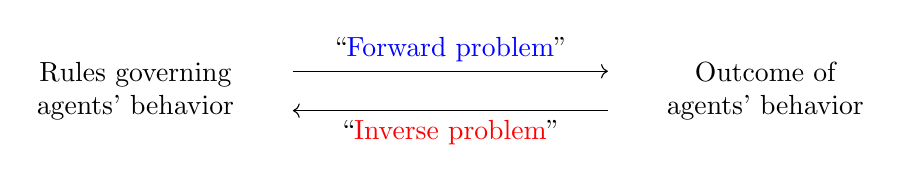
\begin{tikzpicture}
        \node[align=center] at (-2,0) {Rules governing\\agents' behavior};
        \draw[->] (0, 0.25) -- (4, 0.25) node[midway, above] {``\textcolor{blue}{Forward problem}''};
        \draw[<-,visible on=<3->] (0, -0.25) -- (4, -0.25) node[midway, below] {``\textcolor{red}{Inverse problem}''};
        \node[align=center] at (+6,0) {Outcome of\\agents' behavior};
        \end{tikzpicture}
    \end{figure}

    \begin{itemize}
        \item<4-> Inverse problems are \textbf{hard}:
        \begin{enumerate}
            \item<5-> \textbf{Identifiability problems} (underdetermination): many causes could have produced a given outcome
            \item<6-> \textbf{Misspecification problems}: inverse problems may produce misleading results when modeling assumptions are ``too wrong''.
            \item<7-> \textbf{Computational problems}: solving inverse problems often involves intractable computations and requires approximation schemes.
        \end{enumerate}
    \end{itemize}
\end{frame}

\begin{frame}{Bayesian inference for inverse problems}
    \begin{itemize}
        \item Both forward models and inverse problems have a stochastic/probabilistic component (random initialization, partially random decisions, uncertainty quantification\dots)
        \item We appeal to \textbf{probabilities} and \textbf{Bayesian inference}.
    \end{itemize}

    \begin{figure}
        \centering
        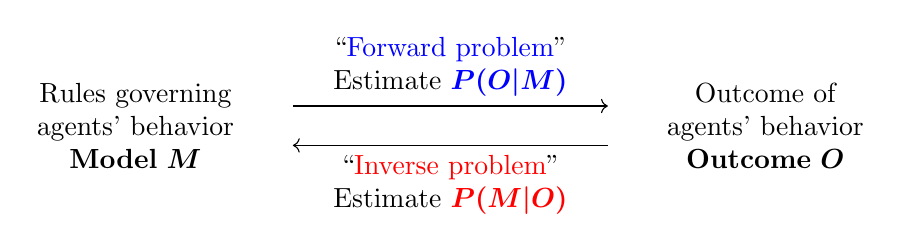
\begin{tikzpicture}
        \node[align=center] at (-2,0) {Rules governing\\agents' behavior\\\textbf{Model} $\bm{M}$};
        \draw[->] (0, 0.25) -- (4, 0.25) node[midway, above, align=center] {``\textcolor{blue}{Forward problem}''\\Estimate $\textcolor{blue}{\bm{P(O|M)}}$};
        \draw[<-] (0, -0.25) -- (4, -0.25) node[midway, below, align=center] {``\textcolor{red}{Inverse problem}''\\Estimate $\textcolor{red}{\bm{P(M|O)}}$};
        \node[align=center] at (+6,0) {Outcome of\\agents' behavior\\\textbf{Outcome} $\bm{O}$};
        \end{tikzpicture}

        \begin{equation}
            \textcolor{red}{P(M|O)} = \dfrac{\textcolor{blue}{P(O|M)}\overbrace{P(M)}^{\text{Prior}}}{P(O)}
        \end{equation}
    \end{figure}
\end{frame}

\begin{frame}{Model comparison and parameter estimation}
    \only<1>{
    \begin{equation}
        \textcolor{red}{P(M|O)} = \dfrac{\textcolor{blue}{P(O|M)}\overbrace{P(M)}^{\text{Prior}}}{P(O)}
    \end{equation}}
    \only<2>{
    \begin{equation}
        \textcolor{red}{P(\theta|O)} = \dfrac{\textcolor{blue}{P(O|\theta)}\overbrace{P(\theta)}^{\text{Prior}}}{P(O)}
    \end{equation}
    }
\end{frame}

\section{A case-study of conventions: the metric signature in particle physics}


\begin{frame}{Conventions}
    \begin{itemize}
        \item<1-> \textbf{Coordination problems} arise when individuals would benefit from acting in a mutually compatible way, but it is somehow non-trivial to do so \citep{Lewis2002}.
        \begin{figure}
        
\begin{tikzpicture}
    % Alice
    \node[alice, minimum size=0.8cm] (alice) at (0,0) {};
    % \node at (0,-1.5) {Alice};

    % Bob
    \node[bob, minimum size=0.8cm] (bob) at (4,0) {};
    % \node at (4,-1.5) {Bob};

    % Phone in the middle
    \node at (2,0) {\faPhone[regular,scale=1.5]};

    % Curly line between Alice and Bob
    \draw[thick, decorate, decoration={snake, amplitude=1mm, segment length=4mm}] 
        (alice.east) -- (1.5,0);
    \draw[thick, decorate, decoration={snake, amplitude=1mm, segment length=4mm}] 
        (2.5,0) -- (bob.west);
    \node[red,visible on=<2->] at (2,0) {\Huge $\times$}; % Red cross in the middle

\end{tikzpicture}

        %     \begin{tikzpicture}
        %         \node[inner sep=0pt,visible on=<1->] (phone) at (0,0)
        % {\includegraphics[width=0.4\textwidth]{presentations/phone.jpg}};
        %         \node[color=red,visible on=<2->] (test) at (0, -0.65) {\HUGE{$\bm{\times}$}};
        
        %     \end{tikzpicture}
        \end{figure}

        \uncover<3->{
            \begin{table}[]
\resizebox{0.5\columnwidth}{!}{%
\begin{tabular}{l|c|c|}
\cline{2-3}
                                                & \textbf{\begin{tabular}[c]{@{}c@{}}Bob\\ calls back\end{tabular}} & \textbf{\begin{tabular}[c]{@{}c@{}}Bob\\ awaits\end{tabular}} \\ \hline
\multicolumn{1}{|l|}{\textbf{Alice calls back}} & 0,0                                                                 & 1,1                                                            \\ \hline
\multicolumn{1}{|l|}{\textbf{Alice awaits}}      & 1,1                                                                 & 0,0                                                            \\ \hline
\end{tabular}%
}
\end{table}
        }
        
        \item<4-> \textbf{``Conventions''} are cultural tools for solving coordination problems by providing individuals with expectations about how others will behave. These expectations suggest particular courses of action.
        \begin{itemize}
            \item<5-> Example: left-hand or right-hand traffic.
            \item<6-> Language! ``The syllable `big' could have meant `small' for all we care, and the red light could have meant `go''' (Quine, foreword to \citealt{Lewis2002})
        \end{itemize}
    \end{itemize}
\end{frame}

\begin{frame}{Conventions in the literature}
\begin{itemize}
    \item<1-> Starting point: conventions as solutions to coordination games \citep{Lewis2002}
    \begin{enumerate}
        \item<2-> Can conventions emerge spontaneously from dyadic interactions alone? \citep{Centola2015,hawkins2019emergence}
        \item<3-> How does the topology of social networks influence the propagation of conventions via dyadic interactions? \citep{pujol2005role,delgado2002emergence}
        \item<4-> How to measure the degree of conventionality of a convention? \citep{OConnor2020}
        \item<5-> What is the role of leadership in addressing coordination problems? \citep{calvert1992leadership}    \end{enumerate}
\end{itemize}
% \begin{itemize}
%     \item Theoretical papers ([evolutionary] game theory, agent-based modeling, e.g. on complex networks\dots)
%     \item Experimental setups.
%     \item Observational analyses of behavioral data (e.g. Twitter data).
% \end{itemize}
\end{frame}

\begin{frame}{A case-study from high-energy physics}
    \begin{itemize}
        \item<1-> Relativistic theories: unified description of spacetime.
        \item<2-> The metric tensor ($g_{\mu\nu})$ captures the metric properties of spacetime; e.g. the pseudo- distance between events $(t_1,x_1,y_1,z_1)$ and $(t_2,x_2,y_2,z_2)$. \textbf{Two possible descriptions} (metric signatures):
    \end{itemize}
    
    \vspace{1em}

    \uncover<3->{
        \begin{equation*}
            \begin{pmatrix}
            +1 & 0 & 0 & 0\\
            0 & -1 & 0 & 0\\
            0 & 0 & -1 & 0\\
            0 & 0 & 0 & -1\\
            \end{pmatrix} \text{ or } \begin{pmatrix}
            -1 & 0 & 0 & 0\\
            0 & +1 & 0 & 0\\
            0 & 0 & +1 & 0\\
            0 & 0 & 0 & +1\\
            \end{pmatrix} ?
        \end{equation*}
    }

    % \uncover<4->{
    %     \begin{equation}
    %         \scriptsize{\Delta s^2 = (t_2-t_1)^2-(x_2-x_1)^2-\dots \text{ or } \Delta s^2 = -(t_2-t_1)^2 +(x_2-x_1)^2+ \dots}
    %     \end{equation}
    % }

    \uncover<4->{
        \begin{equation}
            \text{``mostly minus'' (-1) or ``mostly plus'' (+1)}
        \end{equation}
    }

    \begin{itemize}
        \item<5-> Both choices are legitimate, as long as one remains consistent.
    \end{itemize}
\end{frame}


\begin{frame}{A heated debate}
    \centering
    \begin{tikzpicture}
        \node[inner sep=0pt,visible on=<1->] (meme1) at (0,0)
    {\includegraphics[width=0.55\textwidth]{presentations/meme1.png}};
        \node[inner sep=0pt,visible on=<2->] (meme2) at (2,0)
    {\includegraphics[width=0.45\textwidth]{presentations/meme2.png}};
        \node[inner sep=0pt,visible on=<3->] (meme3) at (0,-2.5)
    {\includegraphics[width=0.45\textwidth]{presentations/meme3.png}};
        \node[inner sep=0pt,visible on=<4->] (meme4) at (-2.5,0)
    {\includegraphics[width=0.45\textwidth]{presentations/meme4.png}};
        \node[inner sep=0pt,visible on=<5->] (meme5) at (0,1.5)
    {\includegraphics[width=0.45\textwidth]{presentations/meme5.png}};
    \end{tikzpicture}
\end{frame}

\begin{frame}{Inverse problems and conventions}
    \begin{itemize}
        \item<1-> Let's use inverse problems to infer:
        \begin{enumerate}
            \item<2-> How do scientists decide which convention to use in a paper?
            \item<3-> How do they resolve conflicting preferences in collaborations?
            \item<4-> What factors shape scientists' preferences?
        \end{enumerate}
    \end{itemize}
\end{frame}

\begin{frame}{Data}
    \begin{itemize}
        \item Data collected from \textbf{Inspire HEP} (authorship/citation metadata) and \textbf{arXiv} (LaTeX source)
        \item Categories: hep-th (high-energy physics theory), hep-ph (phenomenology), gr-qc (gravitation and cosmology), astro-ph (astrophysics)
        \item 22\,500 papers classified according to their metric signature (mostly plus or mostly minus) using regular expressions.
    \end{itemize}
\end{frame}

% \section{Three trade-offs involved in the propagation of conventions}

% \begin{frame}{Trade-offs involved in the diffusion of scientific conventions}
%     \begin{itemize}
%         \item[(A)] Trade-off between \textbf{coordination costs, inconsistency costs, and maladaptation costs}
%         \item[(B)] The competition between \textbf{local and global mechanisms of coordination}
%         \item[(C)] The trade-off between \textbf{decision-optimality} (e.g. collective satisfaction maximization) and \textbf{decision costs}, in the context of the resolution of conflicts.
%     \end{itemize}    
% \end{frame}

\subsection{How do physicists choose which convention to use in their own papers?}

\begin{frame}{How do physicists choose which convention to use in their own papers?}
Individuals' attitude towards a convention may be shaped by:

    \begin{enumerate}
        \item<2-> \textbf{Social consistency} (driven by coordination costs).
        \item<3-> \textbf{Sequential consistency} (driven by switching costs).
        \item<4-> \textbf{Contextual consistency} (the ``maladaptation'' cost of using a convention that is a poor fit/suboptimal in a given context) $\Rightarrow$ degrees of conventionality \citep{OConnor2020}
    \end{enumerate}

    \uncover<5->{$\Rightarrow$ Are these involved in the context of the metric signature? }
\end{frame}

\begin{frame}{Inconsistency and maladaptation costs}
\begin{itemize}
    \item<1-> Is physicists' attitude towards the convention dictated by consistency or adaptation (fitness) to their research?
\end{itemize}

\begin{figure}
\centering
\includegraphics[width=0.5\linewidth]{preferences.pdf}
    \caption{Physicists tend to always be using the same convention}
\end{figure}
\end{frame}

\begin{frame}{Inconsistency and maladaptation costs}
\vspace{-1em}
\def\alice{\tikz[baseline=-.2ex]{
\node[alice] at (0,0) {};}
}

\begin{itemize}
    \item \alice publishes $d$ in category $c_d \in \{\text{phenomenology, theory, \dots}\}$. What is the probability that they use the mostly plus convention?
\end{itemize}

\begin{equation}
    \small P(\sigma_d=+1|a_d=\alice,c_d) = f(\textcolor{red}{\underbrace{\theta(\alice)}_{\substack{\text{Author's}\\\text{preference}}}}+\textcolor{blue}{\underbrace{b(c_d)}_{\substack{\text{Effect of}\\\text{research area } c_d}}})% = \frac{e^{+\frac{1}{2}(\textcolor{red}{\theta_i}+\textcolor{blue}{b_c})}}{e^{+\frac{1}{2}(\textcolor{red}{\theta_i}+\textcolor{blue}{b_c})}+e^{-\frac{1}{2}(\textcolor{red}{\theta_i}+\textcolor{blue}{b_c})}}
\end{equation}

\begin{itemize}
    \item<2-> ``Item-response model'': recover invisible traits/factors that may account for observed behaviors.
    \item<3-> $\theta(i)$ is a latent (unobserved) parameter measuring the preference of each author $i$. $\theta(i)>0$ indicates a preference for the mostly plus signature
    \item<4-> $b_c$ is the unobserved bias associated with research area $c$
    \item<5-> If $|\theta|\gg |b|$ then individual preferences dominate the need to adapt to a given research area
    \item<6-> \textbf{Given physicists' choices in their solo-authored papers, we can infer back $\theta$ and $b$ using Bayesian inference}.
\end{itemize}
\end{frame}

\begin{frame}{Inconsistency and maladaptation costs}
\vspace{-1em}
\begin{figure}
\centering
\includegraphics[width=0.5\linewidth]{consistency_vs_task_barplot.pdf}
    \vspace{-0.75em}
    \caption{Consistency matters the most, but adaptation to the context can occur.}
\end{figure}
\end{frame}



\subsection{How do scientists resolve conflicting preferences in collaborations?}

\begin{frame}{Decision optimality and decision costs in the resolution of conflicts}
    \begin{itemize}
        \item In scientific collaborations, the resolution of disagreement involves two factors:
        \item[1] The ``optimality'' of the decision (i.e., truth-value -- if relevant --, collective satisfaction, appropriateness of the solution etc.).
        \item[2] The cost of reaching an ``optimal'' decision.
        \item Leadership is a tool for reducing ``transaction'' and decision costs in organizations \citep{calvert1992leadership}. Does it play a similar role in the case of the metric signature?
    \end{itemize}
\end{frame}

\begin{frame}{Inferring preference-aggregation mechanisms in conflicts}
    \begin{itemize}
        \item<1-> Focusing on co-authored papers for which:
        \begin{enumerate}
            \item<2->[(i)] The metric signature $S_d\in\{-1,+1\}$ of the paper is observed
            \item<3->[(ii)] The preference of each author $(\sigma_1, \dots, \sigma_n)\in \{\pm 1\}^n$ is known independently from at least one solo-authored publication
            % \item[(iii)] At least two co-authors have conflicting preferences ($\exists i,j | \sigma_i \neq \sigma_j$).
        \end{enumerate}
        \item<4-> We can assume different preference aggregation strategies ($A_k$):
        \begin{itemize}
            \item<5-> Dictatorial strategies (the first author, the last author, or another author decides)
            \item<6-> Majoritarian strategy (the majority preference prevails)
            \item<7-> Conventional strategy (the signature most common in the target research area prevails)
            \item<8-> Random/coin-flip (both individual preferences and context are ignored)
        \end{itemize}
        \item<9-> We can estimate the prevalence of each strategy ($\pi_k$) given that they predict different outcomes (different probabilities  $P(S_d|\sigma_1,\dots,\sigma_n,A_k)$)
    \end{itemize}
\end{frame}

\begin{frame}{Inferring preference-aggregation mechanisms}
    Each paper brings a bit more information about $\pi_k$, the prevalence of an aggregation strategy $A_k$.
        
    \foreach \x in {0,...,59} {
        \newcommand\frameno{\x+1}
        \only<\x>{
            \centering
            \begin{figure}
                \centering
                \includegraphics[width=0.825\linewidth]{aggregation/aggregation_frame_\x.pdf}
            \end{figure}
        }
    }
\end{frame}

\begin{frame}{Prevalence of each preference-aggregation strategy}
    
    \begin{figure}
        \centering
        \includegraphics[width=0.8\linewidth]{aggregation.pdf}
    \end{figure}
\end{frame}

\subsection{How do physicists' preferences get formed?}

\begin{frame}{Authors' preferences ($n=2\,277$)}
    \vspace{-0.75em}
    \begin{figure}[!h]
    \centering
    \includegraphics[width=0.6\textwidth,trim=250 350 225 350,clip]{authors_network.pdf}
    
    \caption{\textbf{Metric signature preferences in the co-author network}. Each node is an author. Edges represent co-authorship relationships between authors. Pink authors have a preference for the mostly minus metric signature, and green authors for the mostly plus metric signature. Only the largest connected component is shown. %Spatialization was performed with ForceAtlas2 \citep{Jacomy2014}.
    }
    \label{fig:co-author-network}
\end{figure}
\end{frame}

\begin{frame}{How do physicists' preferences get formed?}

\begin{itemize}
    \item Let's assume three models of the formation of physicists' preference towards the convention:
    \begin{enumerate}
        \item A \textbf{``strategic agent'' model} ($M_1$) assuming that individuals navigate three costs (coordination costs, inconsistency costs, and maladaptation costs) depending on their collaborators' preferences and the research areas in which they publish.
        \item A \textbf{global cultural transmission model} ($M_2$), in which physicists settle once and for all for a specific convention with a certain probability that depends on their primary research area (textbooks?)
        \item A \textbf{local cultural transmission model} ($M_3$), in which physicists copy the preference of their first collaborator.
    \end{enumerate}
    \item Which of these is more plausible given the observed patterns of preferences?
    % \item We can simulate the processes and measure the magnitudes of local and global coordination that they predict, $P(J,\bm{B}|M)$ and see which of them are consistent with the data!
\end{itemize}
\end{frame}

\begin{frame}{Example: the strategic agent model}
    The model has multiple unknown parameters:
    \begin{itemize}
        \item $c_s$: the cost of switching from one convention to another
        \item $c_c$: the cost of disagreeing with co-authors
        \item $c_{r}$ the cost of using a suboptimal convention in a given research area
    \end{itemize}

    \foreach \x in {0,...,4} {
        \newcommand\frameno{\x+1}
        \only<\x>{
            \centering
            \begin{figure}
                \centering
                \includegraphics[width=0.6\linewidth]{strategic/step_J_\x.pdf}
            \end{figure}
        }
    }
\end{frame}


\begin{frame}{Simulation-based inference}
\vspace{-0.5em}

    \begin{equation}
        \textcolor{red}{P(M_1|O)} = \dfrac{\textcolor{blue}{\overbrace{P(O|M_1)}^{\uncover<2->{\substack{\text{Unknown}\\\text{in ABMs!}}}}}P(M_1)}{P(O)}
    \end{equation}

    % \uncover<2->{
    % Assuming that at least one model is correct:
    % \begin{equation}
    %     P(O) = \displaystyle\sum_{i=1}^3 \textcolor{blue}{P(O|M_i)} P(M_i)
    % \end{equation}
    % }

    \uncover<3->{
    Let us draw $N$ configurations $O_s$, each of them assuming a model $M_s\in\{1,2,3\}$. Then, $\textcolor{blue}{P(O|M_1)}$ is approximated by the fraction of draws from model $M_1$ that match the data:

    \vspace{-0.5em}

    \begin{equation}
        \textcolor{blue}{P(O|M_1)} = \lim_{N\to\infty} \dfrac{\sum_{s=1}^N \mathbbm{1}(O_s=O,M_s=1)}{\sum_{s=1}^N \mathbbm{1}(M_s=1)}
    \end{equation}
    }

    \vspace{-0.5em}
    \uncover<4->{
    \begin{equation}
        \textcolor{red}{P(M_1|O)} = \dfrac{\textcolor{blue}{P(O|M_1)}P(M_1)}{P(O)}\uncover<5->{= \lim_{N\to\infty} \dfrac{\sum_{s=1}^N \mathbbm{1}(O_s=O,M_s=1)}{\sum_{s=1}^N \mathbbm{1}(O_s=O)}} 
    \end{equation}
    }
\end{frame}

\begin{frame}{Curse of dimensionality in simulation-based inference}
    \begin{itemize}
        \item<1-> This approach requires that at least some draws $O_s$ match the observed outcome $O$. These draws must match exactly each and everyone's of the 2\,277 authors' preferences!
        \item<2-> The probability for this to happen is virtually 0 (if a model has a probability $p=0.95$ to predict the correct preference for any author independently, the joint probability would be $2\times 10^{-51}$)
        \item<3-> It would take an absurd amount of time so that at least one simulation matches the observed outcome (many times the age of the universe, even with millions of draws per second)
        \item<4-> This is because because the data has \textit{too many dimensions} $\Rightarrow$ \textbf{``curse of dimensionality''}
        \item<5-> The solution: ``conditioning'' on \textbf{summary statistics} rather than the entire data.
        \item<6-> Summary statistics are \textbf{low-dimensional descriptions of the data} that capture their essential features. e.g.:
        \begin{equation}
            m = \frac{1}{n}|\sum_{i=1}^n \sigma_i|
        \end{equation}
    \end{itemize}
\end{frame}

\begin{frame}{Summary statistics in simulation-based inference}
    There are two main approaches for choosing adequate summary statistics:
    \begin{enumerate}
        \item Hand-picking interpretable summary statistics based on our own intuitions.
        \item Using sophisticated methods to learn statistically optimal (but potentially un-interpretable) summary statistics. Optimal summary statistics reduce our posterior uncertainty given a fixed amount of data.
    \end{enumerate}
\end{frame}

\begin{frame}{Simulation-based inference with summary statistics}
    \foreach \x in {1,...,42} {
        \only<\x>{
            \centering
            \begin{figure}
                \centering
                \includegraphics[width=0.7\linewidth]{abc/frame_\x.pdf}
            \end{figure}
        }
    }
\end{frame}

\begin{frame}{Local versus global mechanisms of coordination}
\begin{figure}
    \centering
    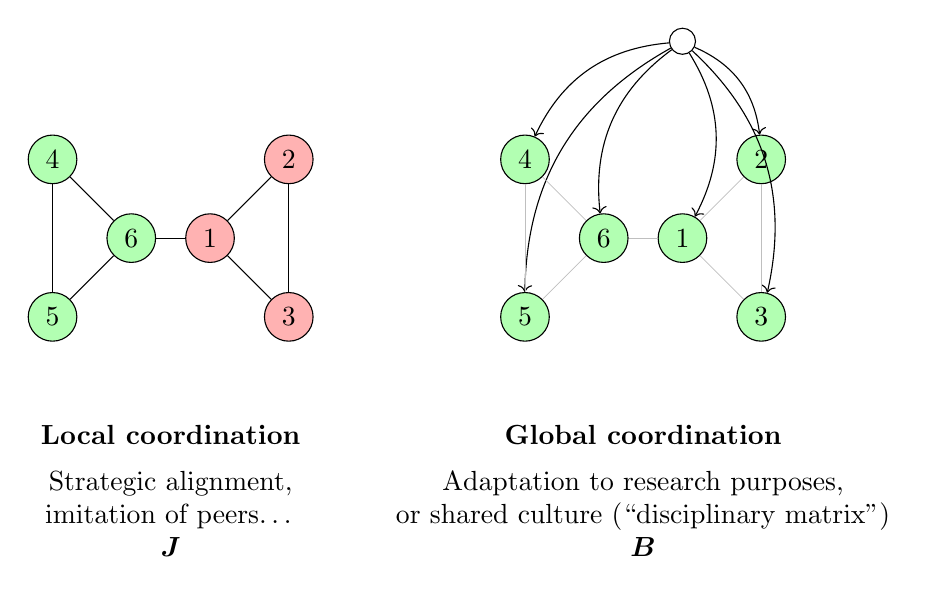
\begin{tikzpicture}
        \node[circle, draw, fill=red!30] (D) at (2,2) {2};
        \node[circle, draw, fill=red!30] (E) at (2,0) {3};
        \node[circle, draw, fill=red!30] (F) at (1,1) {1};
    
        % Left graph (traditional)
        \node[circle, draw, fill=green!30] (A) at (-1,2) {4};
        \node[circle, draw, fill=green!30] (B) at (-1,0) {5};
        \node[circle, draw, fill=green!30] (C) at (0,1) {6};
    
    
        \draw (A) -- (B);
        \draw (B) -- (C);
        \draw (C) -- (A);
        \draw (D) -- (E);
        \draw (E) -- (F);
        \draw (F) -- (D);
    
        \draw (F) -- (C);

        \node[align=center] at (0.5, -1.5) {\textbf{Local coordination}};
        \node[align=center] at (0.5, -2.5) {Strategic alignment,\\imitation of peers\dots\\$\bm{J}$};
    
        % Right graph (common ancestor)
        \node[circle, draw, fill=green!30, visible on=<2->] (D1) at (8,2) {2};
        \node[circle, draw, fill=green!30, visible on=<2->] (E1) at (8,0) {3};
        \node[circle, draw, fill=green!30, visible on=<2->] (F1) at (7,1) {1};
    
        % Left graph (traditional)
        \node[circle, draw, fill=green!30, visible on=<2->] (A1) at (5,2) {4};
        \node[circle, draw, fill=green!30, visible on=<2->] (B1) at (5,0) {5};
        \node[circle, draw, fill=green!30, visible on=<2->] (C1) at (6,1) {6};
        
        \node[circle, draw, visible on=<2->] (Ancestor) at (7,3.5) {};
    
        % Connect the nodes to the common ancestor with curved arrows
        \draw[<-, bend left, visible on=<2->] (A1) to (Ancestor);
        \draw[<-, bend left, visible on=<2->] (B1) to (Ancestor);
        \draw[<-, bend left, visible on=<2->] (C1) to (Ancestor);
        \draw[<-, bend right, visible on=<2->] (D1) to (Ancestor);
        \draw[<-, bend right, visible on=<2->] (E1) to (Ancestor);
        \draw[<-, bend right, visible on=<2->] (F1) to (Ancestor);
    
        \draw[color=gray!50,line width=0.1mm, visible on=<2->] (A1) -- (B1);
        \draw[color=gray!50,line width=0.1mm, visible on=<2->] (B1) -- (C1);
        \draw[color=gray!50,line width=0.1mm, visible on=<2->] (C1) -- (A1);
        \draw[color=gray!50,line width=0.1mm, visible on=<2->] (D1) -- (E1);
        \draw[color=gray!50,line width=0.1mm, visible on=<2->] (E1) -- (F1);
        \draw[color=gray!50,line width=0.1mm, visible on=<2->] (F1) -- (D1);
        \draw[color=gray!50,line width=0.1mm, visible on=<2->] (F1) -- (C1);
        
        \node[align=center, visible on=<2->] at (6.5, -1.5) {\textbf{Global coordination}};
        \node[align=center, visible on=<2->] at (6.5, -2.5) {Adaptation to research purposes,\\ or shared culture (``disciplinary matrix'')\\$\bm{B}$};
    \end{tikzpicture}
\end{figure}
\end{frame}


\begin{frame}{The Ising model as an intermediate idealized model}    
    \begin{itemize}
        \item Atomic magnetic spins in a material can be in two states: $\uparrow$ (+1) or $\downarrow$ (-1).
        \item Magnetic spins prefer to be aligned to their neighbors ($\uparrow\uparrow$ or $\downarrow\downarrow$)
        \item Can local interactions between spins at the microscopic level lead to macroscopic alignment?
    \end{itemize}

    \begin{equation}
    \label{eq:ising}
    P(\{\sigma_i\}|J,\bm{B}) = \frac{1}{Z(J,\bm{B})} e^{-H(\{\sigma_i\},J,\bm{B})}, \text{ and } H = -\underbrace{\sum_{i,j} J w_{ij} \sigma_{i}\sigma_j}_{\substack{\text{local}\\\text{pairwise interactions}}}\underbrace{- \sum_i B_{C_i}\sigma_i}_{\substack{\text{external}\\\text{magnetic field}}}
\end{equation}

\vspace{1em}

\centering
\url{https://mattbierbaum.github.io/ising.js/}

\centering
\vspace{1em}
Inverse Ising problem: $P(J,J^\text{cit},\bm{B}|\{\sigma_i\})$
\end{frame}


\begin{frame}{Local coordination in multi-layered graphs}
    \begin{figure}[!h]
    \centering
\resizebox{0.5\textwidth}{!}{
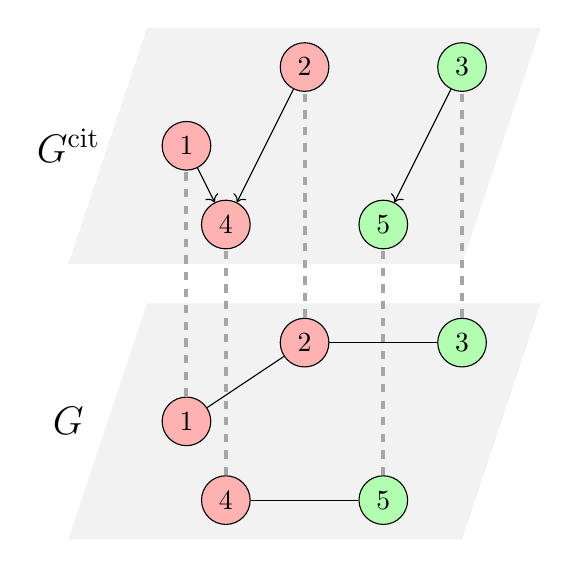
\begin{tikzpicture}
    % Parallelogram for Layer 1 (very transparent gray with more skew)
    \filldraw[fill=gray!10, draw=none] 
    (-2,-0.5) -- (3,-0.5) -- (4,2.5) -- (-1,2.5) -- cycle;

    % Parallelogram for Layer 2 (very transparent gray with more skew)
    \filldraw[fill=gray!10, draw=none] 
    (-2,3) -- (3,3) -- (4,6) -- (-1,6) -- cycle;

    
    % Left graph (traditional)
    \node[circle, draw, fill=red!30] (A) at (0,0) {4};
    \node[circle, draw, fill=green!30] (B) at (2,0) {5};
    \node[circle, draw, fill=red!30] (C) at (1,2) {2};
    \node[circle, draw, fill=green!30] (D) at (3,2) {3};
    \node[circle, draw, fill=red!30] (F) at (-0.5,1) {1};

    \node (g) at (-2,1) {\Large $G$};


    \node[circle, draw, fill=red!30] (A1) at (0,3.5) {4};
    \node[circle, draw, fill=green!30] (B1) at (2,3.5) {5};
    \node[circle, draw, fill=red!30] (C1) at (1,5.5) {2};
    \node[circle, draw, fill=green!30] (D1) at (3,5.5) {3};
    \node[circle, draw, fill=red!30] (F1) at (-0.5,4.5) {1};

    \node (gcit) at (-2,4.5) {\Large $G^{\text{cit}}$};

    \draw (A) -- (B);
    \draw (C) -- (D);
    \draw (C) -- (F);

    \draw[color=gray!70,line width=0.5mm,dashed] (A) -- (A1);
    \draw[color=gray!70,line width=0.5mm,dashed] (B) -- (B1);
    \draw[color=gray!70,line width=0.5mm,dashed] (C) -- (C1);
    \draw[color=gray!70,line width=0.5mm,dashed] (D) -- (D1);
    \draw[color=gray!70,line width=0.5mm,dashed] (F) -- (F1);


    \draw[->] (C1) -- (A1);
    \draw[->] (F1) -- (A1);
    \draw[->] (D1) -- (B1);
    
\end{tikzpicture}
}
\caption{\textbf{Illustration of local coordination in multilayered social networks}. Nodes can be connected through different kinds of relationships (for instance, authors can be related via collaborations ($G$) or citations ($G^{\text{cit}}$)). %In this diagram, patterns of coordination are better explained by the directed graph at the top ($G^{\text{cit}}$): (1,2) have imitated (4), and (3) has imitated (5).
}
    \label{fig:multilayered}
\end{figure}
\end{frame}

\begin{frame}{Local versus global coordination}
\begin{table}[h]
\centering
\caption{Parameters of the Ising model.}
\label{table:ising}
\resizebox{\textwidth}{!}{
\begin{tabular}{lcccc}
\toprule
 & Effect size & CI$_{\text{95\%}}$ & Effect size & CI$_{\text{95\%}}$ \\
Parameter &  &  &  &  \\
\midrule
$J$ & +0.013 & [+0.009, \ +0.017] & +0.0095 & [+0.0052, \ +0.014] \\
$J^{\mathrm{cit}}$ & - & - & +0.00049 & [+0.00023, \ +0.00075] \\
$B(\mathrm{hep-ph})$ & -0.86 & [-0.99, \ -0.73] & -0.77 & [-0.91, \ -0.64] \\
$B(\mathrm{hep-th})$ & -0.22 & [-0.29, \ -0.15] & -0.17 & [-0.24, \ -0.095] \\
$B(\mathrm{gr-qc})$ & +0.075 & [-0.0069, \ +0.16] & +0.076 & [-0.0066, \ +0.16] \\
$B(\mathrm{astro})$ & -0.6 & [-0.74, \ -0.47] & -0.59 & [-0.73, \ -0.46] \\
\bottomrule
\end{tabular}
}
\end{table}
\end{frame}

\begin{frame}{Local versus global coordination}
    What values of $\bm{J}$ and $\bm{B}$ do our models predict? In other words, what is the probability $\textcolor{blue}{P(J,J^\text{cit},\bm{B}|M_i)}$ for each model $M_i$?
    \begin{figure}
        \centering
        \includegraphics[width=0.9\linewidth]{draws_compact_nobars.pdf}
    \end{figure}
\end{frame}

\begin{frame}{Local versus global coordination}
    Given $\textcolor{blue}{P(J,J^\text{cit},\bm{B}|M_i)}$, and the true values of $\bm{J}$ and $\bm{B}$, what is $\textcolor{red}{P(M_i|J,J^{\text{cit}},\bm{B}})$?

    After a bit of computational trickery -- ``amortized simulation-based model comparison with neural networks'' with BayesFlow --:
    
    \begin{figure}
        \centering
        \includegraphics[width=0.9\linewidth]{draws_compact.pdf}
    \end{figure}
\end{frame}

\begin{frame}{Challenges for model selection}
    \begin{itemize}
        \item<1-> Model misspecification: model comparison among highly incorrect models is challenging/meaningless
        \item<2-> Priors on models' parameter matter. A model is disadvantaged if it only is a good fit to the data for improbable parameter values.
    \end{itemize}
\end{frame}

\begin{frame}{Thank you!}
    \nocite{radev2021amortized}
    \printbibliography[heading=none]
\end{frame}

\begin{frame}{Amortized simulation-based inference}
    \begin{itemize}
        \item Even with summary statistics, simulation-based inference is difficult because no simulated sample will \textit{exactly} match the observed data.
        \item Solution:
        \begin{itemize}
            \item<2-> Use amortized inference with neural networks $\Rightarrow$ train a neuralnet to predict the probability of each model $M_i$ given one or more observed outcomes. The neuralnet is trained with many simulated training samples $(M_s, O_s)$ \citep{radev2021amortized}
        \end{itemize}
    \end{itemize}
    \only<3>{
        \centering
        \begin{figure}
            \centering
            \includegraphics[width=0.9\linewidth]{amortized/frame_0.pdf}
        \end{figure}
    }
    \only<4>{
        \centering
        \begin{figure}
            \centering
            \includegraphics[width=0.9\linewidth]{amortized/frame_1.pdf}
        \end{figure}
    }
    \only<5>{
        \centering
        \begin{figure}
            \centering
            \includegraphics[width=0.9\linewidth]{amortized/frame_2.pdf}
        \end{figure}
    }
    \only<6>{
        \centering
        \begin{figure}
            \centering
            \includegraphics[width=0.9\linewidth]{amortized/frame_3.pdf}
        \end{figure}
    }
    \only<7>{
        \centering
        \begin{figure}
            \centering
            \includegraphics[width=0.9\linewidth]{amortized/frame_4.pdf}
        \end{figure}
    }
\end{frame}

\end{document}